\documentclass[twoside]{book}

% Packages required by doxygen
\usepackage{fixltx2e}
\usepackage{calc}
\usepackage{doxygen}
\usepackage{graphicx}
\usepackage[utf8]{inputenc}
\usepackage{makeidx}
\usepackage{multicol}
\usepackage{multirow}
\PassOptionsToPackage{warn}{textcomp}
\usepackage{textcomp}
\usepackage[nointegrals]{wasysym}
\usepackage[table]{xcolor}

% NLS support packages
\usepackage[spanish]{babel}
% Font selection
\usepackage[T1]{fontenc}
\usepackage{mathptmx}
\usepackage[scaled=.90]{helvet}
\usepackage{courier}
\usepackage{amssymb}
\usepackage{sectsty}
\renewcommand{\familydefault}{\sfdefault}
\allsectionsfont{%
  \fontseries{bc}\selectfont%
  \color{darkgray}%
}
\renewcommand{\DoxyLabelFont}{%
  \fontseries{bc}\selectfont%
  \color{darkgray}%
}
\newcommand{\+}{\discretionary{\mbox{\scriptsize$\hookleftarrow$}}{}{}}

% Page & text layout
\usepackage{geometry}
\geometry{%
  a4paper,%
  top=2.5cm,%
  bottom=2.5cm,%
  left=2.5cm,%
  right=2.5cm%
}
\tolerance=750
\hfuzz=15pt
\hbadness=750
\setlength{\emergencystretch}{15pt}
\setlength{\parindent}{0cm}
\setlength{\parskip}{0.2cm}
\makeatletter
\renewcommand{\paragraph}{%
  \@startsection{paragraph}{4}{0ex}{-1.0ex}{1.0ex}{%
    \normalfont\normalsize\bfseries\SS@parafont%
  }%
}
\renewcommand{\subparagraph}{%
  \@startsection{subparagraph}{5}{0ex}{-1.0ex}{1.0ex}{%
    \normalfont\normalsize\bfseries\SS@subparafont%
  }%
}
\makeatother

% Headers & footers
\usepackage{fancyhdr}
\pagestyle{fancyplain}
\fancyhead[LE]{\fancyplain{}{\bfseries\thepage}}
\fancyhead[CE]{\fancyplain{}{}}
\fancyhead[RE]{\fancyplain{}{\bfseries\leftmark}}
\fancyhead[LO]{\fancyplain{}{\bfseries\rightmark}}
\fancyhead[CO]{\fancyplain{}{}}
\fancyhead[RO]{\fancyplain{}{\bfseries\thepage}}
\fancyfoot[LE]{\fancyplain{}{}}
\fancyfoot[CE]{\fancyplain{}{}}
\fancyfoot[RE]{\fancyplain{}{\bfseries\scriptsize Generado el Jueves, 14 de Abril de 2016 17\+:37\+:28 para Laboratorio de P\+R\+O2. Ejercicio '\+Gestión de una lavadora'. por Doxygen }}
\fancyfoot[LO]{\fancyplain{}{\bfseries\scriptsize Generado el Jueves, 14 de Abril de 2016 17\+:37\+:28 para Laboratorio de P\+R\+O2. Ejercicio '\+Gestión de una lavadora'. por Doxygen }}
\fancyfoot[CO]{\fancyplain{}{}}
\fancyfoot[RO]{\fancyplain{}{}}
\renewcommand{\footrulewidth}{0.4pt}
\renewcommand{\chaptermark}[1]{%
  \markboth{#1}{}%
}
\renewcommand{\sectionmark}[1]{%
  \markright{\thesection\ #1}%
}

% Indices & bibliography
\usepackage{natbib}
\usepackage[titles]{tocloft}
\setcounter{tocdepth}{3}
\setcounter{secnumdepth}{5}
\makeindex

% Hyperlinks (required, but should be loaded last)
\usepackage{ifpdf}
\ifpdf
  \usepackage[pdftex,pagebackref=true]{hyperref}
\else
  \usepackage[ps2pdf,pagebackref=true]{hyperref}
\fi
\hypersetup{%
  colorlinks=true,%
  linkcolor=blue,%
  citecolor=blue,%
  unicode%
}

% Custom commands
\newcommand{\clearemptydoublepage}{%
  \newpage{\pagestyle{empty}\cleardoublepage}%
}


%===== C O N T E N T S =====

\begin{document}

% Titlepage & ToC
\hypersetup{pageanchor=false,
             bookmarks=true,
             bookmarksnumbered=true,
             pdfencoding=unicode
            }
\pagenumbering{roman}
\begin{titlepage}
\vspace*{7cm}
\begin{center}%
{\Large Laboratorio de P\+R\+O2. Ejercicio 'Gestión de una lavadora'. \\[1ex]\large version 4 15-\/abr-\/2016 }\\
\vspace*{1cm}
{\large Generado por Doxygen 1.8.8}\\
\vspace*{0.5cm}
{\small Jueves, 14 de Abril de 2016 17:37:28}\\
\end{center}
\end{titlepage}
\clearemptydoublepage
\tableofcontents
\clearemptydoublepage
\pagenumbering{arabic}
\hypersetup{pageanchor=true}

%--- Begin generated contents ---
\chapter{Ejemplo de diseño modular\+: Gestión de una lavadora.}
\label{index}\hypertarget{index}{}El programa principal se encuentra en el módulo \hyperlink{pro2_8cc}{pro2.\+cc}.

Atendiendo a los tipos de datos sugeridos en el enunciado, necesitaremos dos módulos\+: un módulo para representar el almacén y otro para representar una sala.

La simulacion se plantea como un almacén contenedor de un conjunto de salas y un registro de productos global (incluido en el almacén). 
\chapter{Índice de clases}
\section{Lista de clases}
Lista de las clases, estructuras, uniones e interfaces con una breve descripción\+:\begin{DoxyCompactList}
\item\contentsline{section}{\hyperlink{class_cubeta}{Cubeta} \\*Representa una cubeta de ropa }{\pageref{class_cubeta}}{}
\item\contentsline{section}{\hyperlink{class_lavadora}{Lavadora} \\*Representa una lavadora }{\pageref{class_lavadora}}{}
\item\contentsline{section}{\hyperlink{class_prenda}{Prenda} \\*Representa una prenda de ropa con atributos peso y color }{\pageref{class_prenda}}{}
\end{DoxyCompactList}

\chapter{Indice de archivos}
\section{Lista de archivos}
Lista de todos los archivos con descripciones breves\+:\begin{DoxyCompactList}
\item\contentsline{section}{\hyperlink{_cubeta_8hh}{Cubeta.\+hh} \\*Especificación de la clase \hyperlink{class_cubeta}{Cubeta} }{\pageref{_cubeta_8hh}}{}
\item\contentsline{section}{\hyperlink{_lavadora_8hh}{Lavadora.\+hh} \\*Especificación de la clase \hyperlink{class_lavadora}{Lavadora} }{\pageref{_lavadora_8hh}}{}
\item\contentsline{section}{\hyperlink{_prenda_8hh}{Prenda.\+hh} \\*Especificación de la clase \hyperlink{class_prenda}{Prenda} }{\pageref{_prenda_8hh}}{}
\item\contentsline{section}{\hyperlink{pro2__s8_8cc}{pro2\+\_\+s8.\+cc} \\*Programa principal para el ejercicio {\itshape Gestión de una lavadora} }{\pageref{pro2__s8_8cc}}{}
\item\contentsline{section}{\hyperlink{readbool_8hh}{readbool.\+hh} \\*Operacion para leer booleanos del canal estandar }{\pageref{readbool_8hh}}{}
\end{DoxyCompactList}

\chapter{Documentación de las clases}
\hypertarget{class_cubeta}{\section{Referencia de la Clase Cubeta}
\label{class_cubeta}\index{Cubeta@{Cubeta}}
}


Representa una cubeta de ropa.  


\subsection*{Métodos públicos}
\begin{DoxyCompactItemize}
\item 
\hyperlink{class_cubeta_ae85e70c9cd67454446439891e3f435e1}{Cubeta} ()
\begin{DoxyCompactList}\small\item\em Creadora por defecto. \end{DoxyCompactList}\item 
\hyperlink{class_cubeta_a9615e48038899c5732f61661585f12c7}{Cubeta} (const \hyperlink{class_cubeta}{Cubeta} \&c)
\begin{DoxyCompactList}\small\item\em Creadora copiadora. \end{DoxyCompactList}\item 
void \hyperlink{class_cubeta_a431873df8f99cebe56b4787a5271e395}{anadir\+\_\+prenda} (const \hyperlink{class_prenda}{Prenda} \&p)
\begin{DoxyCompactList}\small\item\em Añade una prenda a la cubeta. \end{DoxyCompactList}\item 
void \hyperlink{class_cubeta_a60a5a4f4133ce02f1e4fe49bbe8b9ec7}{completar\+\_\+lavadora} (\hyperlink{class_lavadora}{Lavadora} \&lav)
\begin{DoxyCompactList}\small\item\em Completa una lavadora con las prendas de la cubeta. \end{DoxyCompactList}\item 
void \hyperlink{class_cubeta_a878904c34f1b3361c3913bbaf735ed12}{escribir} () const 
\begin{DoxyCompactList}\small\item\em Operación de escritura. \end{DoxyCompactList}\end{DoxyCompactItemize}


\subsection{Descripción detallada}
Representa una cubeta de ropa. 

Puede contener prendas blancas y de color. Puede usarse para intentar llenar una lavadora; en ese caso, las prendas se sacan de la cubeta en orden inverso al de entrada 

Definición en la línea 21 del archivo Cubeta.\+hh.



\subsection{Documentación del constructor y destructor}
\hypertarget{class_cubeta_ae85e70c9cd67454446439891e3f435e1}{\index{Cubeta@{Cubeta}!Cubeta@{Cubeta}}
\index{Cubeta@{Cubeta}!Cubeta@{Cubeta}}
\subsubsection[{Cubeta}]{\setlength{\rightskip}{0pt plus 5cm}Cubeta\+::\+Cubeta (
\begin{DoxyParamCaption}
{}
\end{DoxyParamCaption}
)}}\label{class_cubeta_ae85e70c9cd67454446439891e3f435e1}


Creadora por defecto. 

Se ejecuta automáticamente al declarar una cubeta. \begin{DoxyPrecond}{Precondición}
{\itshape cierto} 
\end{DoxyPrecond}
\begin{DoxyPostcond}{Postcondición}
El resultado es una cubeta sin prendas de ningún tipo 
\end{DoxyPostcond}
\begin{DoxyParagraph}{Coste}
Constante 
\end{DoxyParagraph}
\hypertarget{class_cubeta_a9615e48038899c5732f61661585f12c7}{\index{Cubeta@{Cubeta}!Cubeta@{Cubeta}}
\index{Cubeta@{Cubeta}!Cubeta@{Cubeta}}
\subsubsection[{Cubeta}]{\setlength{\rightskip}{0pt plus 5cm}Cubeta\+::\+Cubeta (
\begin{DoxyParamCaption}
\item[{const {\bf Cubeta} \&}]{c}
\end{DoxyParamCaption}
)}}\label{class_cubeta_a9615e48038899c5732f61661585f12c7}


Creadora copiadora. 

Permite declarar una cubeta nueva como copia de otra ya existente. \begin{DoxyPrecond}{Precondición}
{\itshape cierto} 
\end{DoxyPrecond}
\begin{DoxyPostcond}{Postcondición}
El resultado es una cubeta igual que c 
\end{DoxyPostcond}
\begin{DoxyParagraph}{Coste}
Lineal respecto al número de prendas de c 
\end{DoxyParagraph}


\subsection{Documentación de las funciones miembro}
\hypertarget{class_cubeta_a431873df8f99cebe56b4787a5271e395}{\index{Cubeta@{Cubeta}!anadir\+\_\+prenda@{anadir\+\_\+prenda}}
\index{anadir\+\_\+prenda@{anadir\+\_\+prenda}!Cubeta@{Cubeta}}
\subsubsection[{anadir\+\_\+prenda}]{\setlength{\rightskip}{0pt plus 5cm}void Cubeta\+::anadir\+\_\+prenda (
\begin{DoxyParamCaption}
\item[{const {\bf Prenda} \&}]{p}
\end{DoxyParamCaption}
)}}\label{class_cubeta_a431873df8f99cebe56b4787a5271e395}


Añade una prenda a la cubeta. 

\begin{DoxyPrecond}{Precondición}
{\itshape cierto} 
\end{DoxyPrecond}
\begin{DoxyPostcond}{Postcondición}
El parámetro implícito pasa a contener sus prendas originales más p 
\end{DoxyPostcond}
\begin{DoxyParagraph}{Coste}
Constante 
\end{DoxyParagraph}
\hypertarget{class_cubeta_a60a5a4f4133ce02f1e4fe49bbe8b9ec7}{\index{Cubeta@{Cubeta}!completar\+\_\+lavadora@{completar\+\_\+lavadora}}
\index{completar\+\_\+lavadora@{completar\+\_\+lavadora}!Cubeta@{Cubeta}}
\subsubsection[{completar\+\_\+lavadora}]{\setlength{\rightskip}{0pt plus 5cm}void Cubeta\+::completar\+\_\+lavadora (
\begin{DoxyParamCaption}
\item[{{\bf Lavadora} \&}]{lav}
\end{DoxyParamCaption}
)}}\label{class_cubeta_a60a5a4f4133ce02f1e4fe49bbe8b9ec7}


Completa una lavadora con las prendas de la cubeta. 

\begin{DoxyPrecond}{Precondición}
lav está inicializada 
\end{DoxyPrecond}
\begin{DoxyPostcond}{Postcondición}
Se han eliminado del parámetro implícito y se han añadido a lav las prendas del parámetro implícito del color adecuado que más se acercan entre todas al peso máximo de lav sin pasarse, elegiéndose primero las que se introdujeron en último lugar 
\end{DoxyPostcond}
\begin{DoxyParagraph}{Coste}
Lineal respecto al número de prendas del parámetro implícito 
\end{DoxyParagraph}
\hypertarget{class_cubeta_a878904c34f1b3361c3913bbaf735ed12}{\index{Cubeta@{Cubeta}!escribir@{escribir}}
\index{escribir@{escribir}!Cubeta@{Cubeta}}
\subsubsection[{escribir}]{\setlength{\rightskip}{0pt plus 5cm}void Cubeta\+::escribir (
\begin{DoxyParamCaption}
{}
\end{DoxyParamCaption}
) const}}\label{class_cubeta_a878904c34f1b3361c3913bbaf735ed12}


Operación de escritura. 

\begin{DoxyPrecond}{Precondición}
{\itshape cierto} 
\end{DoxyPrecond}
\begin{DoxyPostcond}{Postcondición}
Escribe el contenido del parámetro implícito por el canal estándar de salida 
\end{DoxyPostcond}
\begin{DoxyParagraph}{Coste}
Lineal respecto al número de prendas del parámetro implícito 
\end{DoxyParagraph}


La documentación para esta clase fue generada a partir del siguiente fichero\+:\begin{DoxyCompactItemize}
\item 
\hyperlink{_cubeta_8hh}{Cubeta.\+hh}\end{DoxyCompactItemize}

\hypertarget{class_lavadora}{\section{Referencia de la Clase Lavadora}
\label{class_lavadora}\index{Lavadora@{Lavadora}}
}


Representa una lavadora.  


\subsection*{Métodos públicos}
\begin{DoxyCompactItemize}
\item 
\hyperlink{class_lavadora_a2366b1cd0ba86f8ef8ba8504067dc114}{Lavadora} ()
\begin{DoxyCompactList}\small\item\em Creadora por defecto. \end{DoxyCompactList}\item 
void \hyperlink{class_lavadora_a733af02910dca3f75390be4ca6ac84f6}{inicializar} (int pmax, bool col)
\begin{DoxyCompactList}\small\item\em Inicializa la lavadora. \end{DoxyCompactList}\item 
void \hyperlink{class_lavadora_a7e465e1f11ba5ba3cffcee1ce9507e79}{anadir\+\_\+prenda} (const \hyperlink{class_prenda}{Prenda} \&p)
\begin{DoxyCompactList}\small\item\em Añade una prenda a la lavadora. \end{DoxyCompactList}\item 
void \hyperlink{class_lavadora_a82bd403e688482030fcb95f0c3fd62d1}{lavado} ()
\begin{DoxyCompactList}\small\item\em Realiza un lavado. \end{DoxyCompactList}\item 
bool \hyperlink{class_lavadora_a0788f5869b65672123a0f53f278b6165}{esta\+\_\+inicializada} () const 
\begin{DoxyCompactList}\small\item\em Consultora del estado de la lavadora. \end{DoxyCompactList}\item 
bool \hyperlink{class_lavadora_a0f1a4951efc12b14052463e1a317b5a7}{consultar\+\_\+color} () const 
\begin{DoxyCompactList}\small\item\em Consultora del color de la lavadora. \end{DoxyCompactList}\item 
int \hyperlink{class_lavadora_a062c958e69eeda22bf34cea2e6d5212e}{consultar\+\_\+peso} () const 
\begin{DoxyCompactList}\small\item\em Consultora del peso actual de la lavadora. \end{DoxyCompactList}\item 
int \hyperlink{class_lavadora_a9e687c3d38303e79ae5aea620d074a68}{consultar\+\_\+peso\+\_\+maximo} () const 
\begin{DoxyCompactList}\small\item\em Consultora del peso máximo de la lavadora. \end{DoxyCompactList}\item 
void \hyperlink{class_lavadora_a137b1b3b53ce1cce3b3d112616b4a247}{escribir} () const 
\begin{DoxyCompactList}\small\item\em Operación de escritura. \end{DoxyCompactList}\end{DoxyCompactItemize}


\subsection{Descripción detallada}
Representa una lavadora. 

Dispone de dos estados posibles (inicializada / no inicializada); si está inicializada tiene un peso máximo y un color y puede contener prendas de dicho color hasta alcanzar dicho peso máximo; si no está inicializada no contiene ninguna prenda y solo se puede inicializar

Todas las operaciones son de {\bfseries coste constante} salvo las indicadas 

Definición en la línea 20 del archivo Lavadora.\+hh.



\subsection{Documentación del constructor y destructor}
\hypertarget{class_lavadora_a2366b1cd0ba86f8ef8ba8504067dc114}{\index{Lavadora@{Lavadora}!Lavadora@{Lavadora}}
\index{Lavadora@{Lavadora}!Lavadora@{Lavadora}}
\subsubsection[{Lavadora}]{\setlength{\rightskip}{0pt plus 5cm}Lavadora\+::\+Lavadora (
\begin{DoxyParamCaption}
{}
\end{DoxyParamCaption}
)}}\label{class_lavadora_a2366b1cd0ba86f8ef8ba8504067dc114}


Creadora por defecto. 

Se ejecuta automáticamente al declarar una lavadora. \begin{DoxyPrecond}{Precondición}
{\itshape cierto} 
\end{DoxyPrecond}
\begin{DoxyPostcond}{Postcondición}
El resultado es una lavadora no inicializada 
\end{DoxyPostcond}


\subsection{Documentación de las funciones miembro}
\hypertarget{class_lavadora_a733af02910dca3f75390be4ca6ac84f6}{\index{Lavadora@{Lavadora}!inicializar@{inicializar}}
\index{inicializar@{inicializar}!Lavadora@{Lavadora}}
\subsubsection[{inicializar}]{\setlength{\rightskip}{0pt plus 5cm}void Lavadora\+::inicializar (
\begin{DoxyParamCaption}
\item[{int}]{pmax, }
\item[{bool}]{col}
\end{DoxyParamCaption}
)}}\label{class_lavadora_a733af02910dca3f75390be4ca6ac84f6}


Inicializa la lavadora. 

\begin{DoxyPrecond}{Precondición}
El parámetro implícito no está inicializado, pmax$>$0 
\end{DoxyPrecond}
\begin{DoxyPostcond}{Postcondición}
El parámetro implícito pasa a estar inicializado con peso máximo \char`\"{}pmax\char`\"{} y color \char`\"{}col\char`\"{} 
\end{DoxyPostcond}
\hypertarget{class_lavadora_a7e465e1f11ba5ba3cffcee1ce9507e79}{\index{Lavadora@{Lavadora}!anadir\+\_\+prenda@{anadir\+\_\+prenda}}
\index{anadir\+\_\+prenda@{anadir\+\_\+prenda}!Lavadora@{Lavadora}}
\subsubsection[{anadir\+\_\+prenda}]{\setlength{\rightskip}{0pt plus 5cm}void Lavadora\+::anadir\+\_\+prenda (
\begin{DoxyParamCaption}
\item[{const {\bf Prenda} \&}]{p}
\end{DoxyParamCaption}
)}}\label{class_lavadora_a7e465e1f11ba5ba3cffcee1ce9507e79}


Añade una prenda a la lavadora. 

\begin{DoxyPrecond}{Precondición}
El parámetro implícito (L) está inicializado, color de p = color de L, peso de L + peso de p $<$= peso máximo de L 
\end{DoxyPrecond}
\begin{DoxyPostcond}{Postcondición}
El parámetro implícito contiene su carga original más p 
\end{DoxyPostcond}
\hypertarget{class_lavadora_a82bd403e688482030fcb95f0c3fd62d1}{\index{Lavadora@{Lavadora}!lavado@{lavado}}
\index{lavado@{lavado}!Lavadora@{Lavadora}}
\subsubsection[{lavado}]{\setlength{\rightskip}{0pt plus 5cm}void Lavadora\+::lavado (
\begin{DoxyParamCaption}
{}
\end{DoxyParamCaption}
)}}\label{class_lavadora_a82bd403e688482030fcb95f0c3fd62d1}


Realiza un lavado. 

Representa que se realiza el lavado, se retiran la prendas que contiene la lavadora y ésta queda en estado de volver a usarse \begin{DoxyPrecond}{Precondición}
El parámetro implícito está inicializado 
\end{DoxyPrecond}
\begin{DoxyPostcond}{Postcondición}
El parámetro implícito no está inicializado 
\end{DoxyPostcond}
\begin{DoxyParagraph}{Coste}
Lineal respecto al número de prendas del parámetro implícito 
\end{DoxyParagraph}
\hypertarget{class_lavadora_a0788f5869b65672123a0f53f278b6165}{\index{Lavadora@{Lavadora}!esta\+\_\+inicializada@{esta\+\_\+inicializada}}
\index{esta\+\_\+inicializada@{esta\+\_\+inicializada}!Lavadora@{Lavadora}}
\subsubsection[{esta\+\_\+inicializada}]{\setlength{\rightskip}{0pt plus 5cm}bool Lavadora\+::esta\+\_\+inicializada (
\begin{DoxyParamCaption}
{}
\end{DoxyParamCaption}
) const}}\label{class_lavadora_a0788f5869b65672123a0f53f278b6165}


Consultora del estado de la lavadora. 

\begin{DoxyPrecond}{Precondición}
{\itshape cierto} 
\end{DoxyPrecond}
\begin{DoxyPostcond}{Postcondición}
El resultado indica si el parámetro implícito está inicializado 
\end{DoxyPostcond}
\hypertarget{class_lavadora_a0f1a4951efc12b14052463e1a317b5a7}{\index{Lavadora@{Lavadora}!consultar\+\_\+color@{consultar\+\_\+color}}
\index{consultar\+\_\+color@{consultar\+\_\+color}!Lavadora@{Lavadora}}
\subsubsection[{consultar\+\_\+color}]{\setlength{\rightskip}{0pt plus 5cm}bool Lavadora\+::consultar\+\_\+color (
\begin{DoxyParamCaption}
{}
\end{DoxyParamCaption}
) const}}\label{class_lavadora_a0f1a4951efc12b14052463e1a317b5a7}


Consultora del color de la lavadora. 

\begin{DoxyPrecond}{Precondición}
El parámetro implícito está inicializado 
\end{DoxyPrecond}
\begin{DoxyPostcond}{Postcondición}
El resultado es el color del parámetro implícito 
\end{DoxyPostcond}
\hypertarget{class_lavadora_a062c958e69eeda22bf34cea2e6d5212e}{\index{Lavadora@{Lavadora}!consultar\+\_\+peso@{consultar\+\_\+peso}}
\index{consultar\+\_\+peso@{consultar\+\_\+peso}!Lavadora@{Lavadora}}
\subsubsection[{consultar\+\_\+peso}]{\setlength{\rightskip}{0pt plus 5cm}int Lavadora\+::consultar\+\_\+peso (
\begin{DoxyParamCaption}
{}
\end{DoxyParamCaption}
) const}}\label{class_lavadora_a062c958e69eeda22bf34cea2e6d5212e}


Consultora del peso actual de la lavadora. 

\begin{DoxyPrecond}{Precondición}
El parámetro implícito está inicializado 
\end{DoxyPrecond}
\begin{DoxyPostcond}{Postcondición}
El resultado es la suma de los pesos de las prendas del parámetro implícito 
\end{DoxyPostcond}
\hypertarget{class_lavadora_a9e687c3d38303e79ae5aea620d074a68}{\index{Lavadora@{Lavadora}!consultar\+\_\+peso\+\_\+maximo@{consultar\+\_\+peso\+\_\+maximo}}
\index{consultar\+\_\+peso\+\_\+maximo@{consultar\+\_\+peso\+\_\+maximo}!Lavadora@{Lavadora}}
\subsubsection[{consultar\+\_\+peso\+\_\+maximo}]{\setlength{\rightskip}{0pt plus 5cm}int Lavadora\+::consultar\+\_\+peso\+\_\+maximo (
\begin{DoxyParamCaption}
{}
\end{DoxyParamCaption}
) const}}\label{class_lavadora_a9e687c3d38303e79ae5aea620d074a68}


Consultora del peso máximo de la lavadora. 

\begin{DoxyPrecond}{Precondición}
El parámetro implícito está inicializado 
\end{DoxyPrecond}
\begin{DoxyPostcond}{Postcondición}
El resultado es el peso máximo del parámetro implícito 
\end{DoxyPostcond}
\hypertarget{class_lavadora_a137b1b3b53ce1cce3b3d112616b4a247}{\index{Lavadora@{Lavadora}!escribir@{escribir}}
\index{escribir@{escribir}!Lavadora@{Lavadora}}
\subsubsection[{escribir}]{\setlength{\rightskip}{0pt plus 5cm}void Lavadora\+::escribir (
\begin{DoxyParamCaption}
{}
\end{DoxyParamCaption}
) const}}\label{class_lavadora_a137b1b3b53ce1cce3b3d112616b4a247}


Operación de escritura. 

\begin{DoxyPrecond}{Precondición}
El parámetro implícito está inicializado 
\end{DoxyPrecond}
\begin{DoxyPostcond}{Postcondición}
Escribe las propiedades y el contenido del parámetro implícito por el canal estándar de salida 
\end{DoxyPostcond}
\begin{DoxyParagraph}{Coste}
Lineal respecto al número de prendas del parámetro implícito 
\end{DoxyParagraph}


La documentación para esta clase fue generada a partir del siguiente fichero\+:\begin{DoxyCompactItemize}
\item 
\hyperlink{_lavadora_8hh}{Lavadora.\+hh}\end{DoxyCompactItemize}

\hypertarget{class_prenda}{\section{Referencia de la Clase Prenda}
\label{class_prenda}\index{Prenda@{Prenda}}
}


Representa una prenda de ropa con atributos peso y color.  


\subsection*{Métodos públicos}
\begin{DoxyCompactItemize}
\item 
\hyperlink{class_prenda_adfd86b131c7f40c58b0cb4200eb55129}{Prenda} ()
\begin{DoxyCompactList}\small\item\em Creadora por defecto. \end{DoxyCompactList}\item 
\hyperlink{class_prenda_af15ff723083040b89bc495b4ec4b914e}{Prenda} (int pes, bool col)
\begin{DoxyCompactList}\small\item\em Creadora con valores concretos. \end{DoxyCompactList}\item 
void \hyperlink{class_prenda_ab25b2a66034eb2c0fccfb1f3cedbb5a7}{modificar} (int pes, bool col)
\begin{DoxyCompactList}\small\item\em Modificadora de los atributos. \end{DoxyCompactList}\item 
int \hyperlink{class_prenda_ae886133326d46cc18dd9070d317a3ccb}{consul\+\_\+peso} () const 
\begin{DoxyCompactList}\small\item\em Consultora del peso. \end{DoxyCompactList}\item 
bool \hyperlink{class_prenda_a149632ba71127621c52917ef2e936c2e}{consul\+\_\+color} () const 
\begin{DoxyCompactList}\small\item\em Consultora del color. \end{DoxyCompactList}\item 
void \hyperlink{class_prenda_a3a5dfb75467c54157ec969b8ab7d752b}{escribir} () const 
\begin{DoxyCompactList}\small\item\em Operación de escritura. \end{DoxyCompactList}\end{DoxyCompactItemize}


\subsection{Descripción detallada}
Representa una prenda de ropa con atributos peso y color. 

Todas las operaciones son de {\bfseries coste constante} 

Definición en la línea 19 del archivo Prenda.\+hh.



\subsection{Documentación del constructor y destructor}
\hypertarget{class_prenda_adfd86b131c7f40c58b0cb4200eb55129}{\index{Prenda@{Prenda}!Prenda@{Prenda}}
\index{Prenda@{Prenda}!Prenda@{Prenda}}
\subsubsection[{Prenda}]{\setlength{\rightskip}{0pt plus 5cm}Prenda\+::\+Prenda (
\begin{DoxyParamCaption}
{}
\end{DoxyParamCaption}
)}}\label{class_prenda_adfd86b131c7f40c58b0cb4200eb55129}


Creadora por defecto. 

Se ejecuta automáticamente al declarar una prenda. \begin{DoxyPrecond}{Precondición}
{\itshape cierto} 
\end{DoxyPrecond}
\begin{DoxyPostcond}{Postcondición}
El resultado es una prenda de peso 0 y color blanco 
\end{DoxyPostcond}
\hypertarget{class_prenda_af15ff723083040b89bc495b4ec4b914e}{\index{Prenda@{Prenda}!Prenda@{Prenda}}
\index{Prenda@{Prenda}!Prenda@{Prenda}}
\subsubsection[{Prenda}]{\setlength{\rightskip}{0pt plus 5cm}Prenda\+::\+Prenda (
\begin{DoxyParamCaption}
\item[{int}]{pes, }
\item[{bool}]{col}
\end{DoxyParamCaption}
)}}\label{class_prenda_af15ff723083040b89bc495b4ec4b914e}


Creadora con valores concretos. 

\begin{DoxyPrecond}{Precondición}
pes$>$0 
\end{DoxyPrecond}
\begin{DoxyPostcond}{Postcondición}
El resultado es una prenda con peso \char`\"{}pes\char`\"{} y color \char`\"{}col\char`\"{} 
\end{DoxyPostcond}


\subsection{Documentación de las funciones miembro}
\hypertarget{class_prenda_ab25b2a66034eb2c0fccfb1f3cedbb5a7}{\index{Prenda@{Prenda}!modificar@{modificar}}
\index{modificar@{modificar}!Prenda@{Prenda}}
\subsubsection[{modificar}]{\setlength{\rightskip}{0pt plus 5cm}void Prenda\+::modificar (
\begin{DoxyParamCaption}
\item[{int}]{pes, }
\item[{bool}]{col}
\end{DoxyParamCaption}
)}}\label{class_prenda_ab25b2a66034eb2c0fccfb1f3cedbb5a7}


Modificadora de los atributos. 

\begin{DoxyPrecond}{Precondición}
pes$>$0 
\end{DoxyPrecond}
\begin{DoxyPostcond}{Postcondición}
El parámetro implícito pasa a tener peso \char`\"{}pes\char`\"{} y color \char`\"{}col\char`\"{} 
\end{DoxyPostcond}
\hypertarget{class_prenda_ae886133326d46cc18dd9070d317a3ccb}{\index{Prenda@{Prenda}!consul\+\_\+peso@{consul\+\_\+peso}}
\index{consul\+\_\+peso@{consul\+\_\+peso}!Prenda@{Prenda}}
\subsubsection[{consul\+\_\+peso}]{\setlength{\rightskip}{0pt plus 5cm}int Prenda\+::consul\+\_\+peso (
\begin{DoxyParamCaption}
{}
\end{DoxyParamCaption}
) const}}\label{class_prenda_ae886133326d46cc18dd9070d317a3ccb}


Consultora del peso. 

\begin{DoxyPrecond}{Precondición}
{\itshape cierto} 
\end{DoxyPrecond}
\begin{DoxyPostcond}{Postcondición}
El resultado es el peso del parámetro implícito 
\end{DoxyPostcond}
\hypertarget{class_prenda_a149632ba71127621c52917ef2e936c2e}{\index{Prenda@{Prenda}!consul\+\_\+color@{consul\+\_\+color}}
\index{consul\+\_\+color@{consul\+\_\+color}!Prenda@{Prenda}}
\subsubsection[{consul\+\_\+color}]{\setlength{\rightskip}{0pt plus 5cm}bool Prenda\+::consul\+\_\+color (
\begin{DoxyParamCaption}
{}
\end{DoxyParamCaption}
) const}}\label{class_prenda_a149632ba71127621c52917ef2e936c2e}


Consultora del color. 

\begin{DoxyPrecond}{Precondición}
{\itshape cierto} 
\end{DoxyPrecond}
\begin{DoxyPostcond}{Postcondición}
El resultado es el color del parámetro implícito 
\end{DoxyPostcond}
\hypertarget{class_prenda_a3a5dfb75467c54157ec969b8ab7d752b}{\index{Prenda@{Prenda}!escribir@{escribir}}
\index{escribir@{escribir}!Prenda@{Prenda}}
\subsubsection[{escribir}]{\setlength{\rightskip}{0pt plus 5cm}void Prenda\+::escribir (
\begin{DoxyParamCaption}
{}
\end{DoxyParamCaption}
) const}}\label{class_prenda_a3a5dfb75467c54157ec969b8ab7d752b}


Operación de escritura. 

\begin{DoxyPrecond}{Precondición}
{\itshape cierto} 
\end{DoxyPrecond}
\begin{DoxyPostcond}{Postcondición}
Se han escrito los atributos del parámetro implícito en el canal standard de salida. 
\end{DoxyPostcond}


La documentación para esta clase fue generada a partir del siguiente fichero\+:\begin{DoxyCompactItemize}
\item 
\hyperlink{_prenda_8hh}{Prenda.\+hh}\end{DoxyCompactItemize}

\chapter{Documentación de archivos}
\hypertarget{_cubeta_8hh}{\section{Referencia del Archivo Cubeta.\+hh}
\label{_cubeta_8hh}\index{Cubeta.\+hh@{Cubeta.\+hh}}
}


Especificación de la clase \hyperlink{class_cubeta}{Cubeta}.  


Dependencia gráfica adjunta para Cubeta.\+hh\+:\nopagebreak
\begin{figure}[H]
\begin{center}
\leavevmode
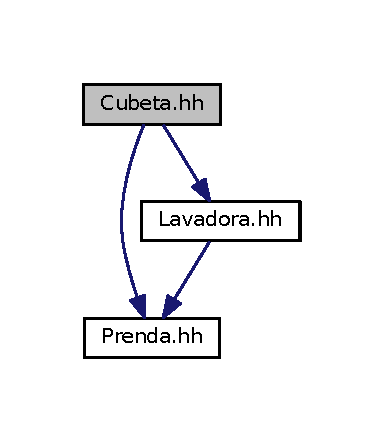
\includegraphics[width=184pt]{_cubeta_8hh__incl}
\end{center}
\end{figure}
\subsection*{Clases}
\begin{DoxyCompactItemize}
\item 
class \hyperlink{class_cubeta}{Cubeta}
\begin{DoxyCompactList}\small\item\em Representa una cubeta de ropa. \end{DoxyCompactList}\end{DoxyCompactItemize}


\subsection{Descripción detallada}
Especificación de la clase \hyperlink{class_cubeta}{Cubeta}. 



Definición en el archivo \hyperlink{_cubeta_8hh_source}{Cubeta.\+hh}.


\hypertarget{_lavadora_8hh}{\section{Referencia del Archivo Lavadora.\+hh}
\label{_lavadora_8hh}\index{Lavadora.\+hh@{Lavadora.\+hh}}
}


Especificación de la clase \hyperlink{class_lavadora}{Lavadora}.  


Dependencia gráfica adjunta para Lavadora.\+hh\+:\nopagebreak
\begin{figure}[H]
\begin{center}
\leavevmode
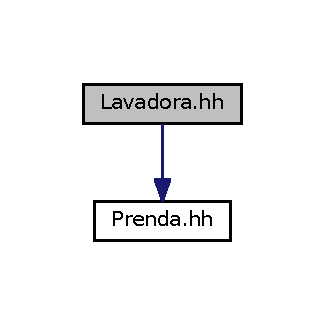
\includegraphics[width=156pt]{_lavadora_8hh__incl}
\end{center}
\end{figure}
\subsection*{Clases}
\begin{DoxyCompactItemize}
\item 
class \hyperlink{class_lavadora}{Lavadora}
\begin{DoxyCompactList}\small\item\em Representa una lavadora. \end{DoxyCompactList}\end{DoxyCompactItemize}


\subsection{Descripción detallada}
Especificación de la clase \hyperlink{class_lavadora}{Lavadora}. 



Definición en el archivo \hyperlink{_lavadora_8hh_source}{Lavadora.\+hh}.


\hypertarget{_prenda_8hh}{\section{Referencia del Archivo Prenda.\+hh}
\label{_prenda_8hh}\index{Prenda.\+hh@{Prenda.\+hh}}
}


Especificación de la clase \hyperlink{class_prenda}{Prenda}.  


\subsection*{Clases}
\begin{DoxyCompactItemize}
\item 
class \hyperlink{class_prenda}{Prenda}
\begin{DoxyCompactList}\small\item\em Representa una prenda de ropa con atributos peso y color. \end{DoxyCompactList}\end{DoxyCompactItemize}


\subsection{Descripción detallada}
Especificación de la clase \hyperlink{class_prenda}{Prenda}. 



Definición en el archivo \hyperlink{_prenda_8hh_source}{Prenda.\+hh}.


\hypertarget{pro2__s8_8cc}{\section{Referencia del Archivo pro2\+\_\+s8.\+cc}
\label{pro2__s8_8cc}\index{pro2\+\_\+s8.\+cc@{pro2\+\_\+s8.\+cc}}
}


Programa principal para el ejercicio {\itshape Gestión de una lavadora}.  


Dependencia gráfica adjunta para pro2\+\_\+s8.\+cc\+:\nopagebreak
\begin{figure}[H]
\begin{center}
\leavevmode
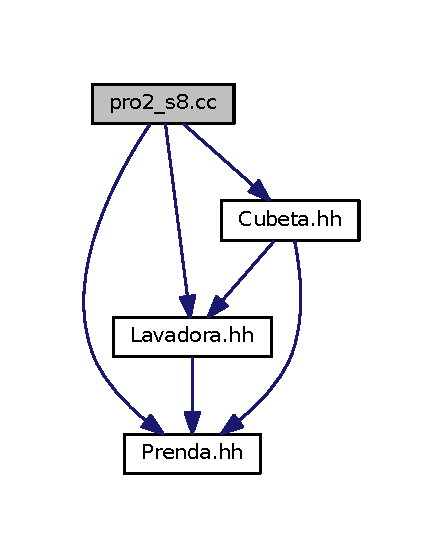
\includegraphics[width=212pt]{pro2__s8_8cc__incl}
\end{center}
\end{figure}
\subsection*{Funciones}
\begin{DoxyCompactItemize}
\item 
int \hyperlink{pro2__s8_8cc_ae66f6b31b5ad750f1fe042a706a4e3d4}{main} ()
\begin{DoxyCompactList}\small\item\em Programa principal para el ejercicio {\itshape Gestión de una lavadora}. \end{DoxyCompactList}\end{DoxyCompactItemize}


\subsection{Descripción detallada}
Programa principal para el ejercicio {\itshape Gestión de una lavadora}. 



Definición en el archivo \hyperlink{pro2__s8_8cc_source}{pro2\+\_\+s8.\+cc}.



\subsection{Documentación de las funciones}
\hypertarget{pro2__s8_8cc_ae66f6b31b5ad750f1fe042a706a4e3d4}{\index{pro2\+\_\+s8.\+cc@{pro2\+\_\+s8.\+cc}!main@{main}}
\index{main@{main}!pro2\+\_\+s8.\+cc@{pro2\+\_\+s8.\+cc}}
\subsubsection[{main}]{\setlength{\rightskip}{0pt plus 5cm}int main (
\begin{DoxyParamCaption}
{}
\end{DoxyParamCaption}
)}}\label{pro2__s8_8cc_ae66f6b31b5ad750f1fe042a706a4e3d4}


Programa principal para el ejercicio {\itshape Gestión de una lavadora}. 



Definición en la línea 25 del archivo pro2\+\_\+s8.\+cc.


\begin{DoxyCode}
26 \{
27 
28 \}
\end{DoxyCode}

\hypertarget{readbool_8hh}{\section{Referencia del Archivo readbool.\+hh}
\label{readbool_8hh}\index{readbool.\+hh@{readbool.\+hh}}
}


operacion para leer booleanos del canal estandar  


\subsection*{Funciones}
\begin{DoxyCompactItemize}
\item 
bool \hyperlink{readbool_8hh_a56691e176645da552c107ef124ad701a}{readbool} ()
\begin{DoxyCompactList}\small\item\em Lee un booleano por el canal estandar. \end{DoxyCompactList}\end{DoxyCompactItemize}


\subsection{Descripción detallada}
operacion para leer booleanos del canal estandar 



Definición en el archivo \hyperlink{readbool_8hh_source}{readbool.\+hh}.



\subsection{Documentación de las funciones}
\hypertarget{readbool_8hh_a56691e176645da552c107ef124ad701a}{\index{readbool.\+hh@{readbool.\+hh}!readbool@{readbool}}
\index{readbool@{readbool}!readbool.\+hh@{readbool.\+hh}}
\subsubsection[{readbool}]{\setlength{\rightskip}{0pt plus 5cm}bool readbool (
\begin{DoxyParamCaption}
{}
\end{DoxyParamCaption}
)}}\label{readbool_8hh_a56691e176645da552c107ef124ad701a}


Lee un booleano por el canal estandar. 

\begin{DoxyPrecond}{Precondición}
La primera string valida del canal estandar es \char`\"{}true\char`\"{} o \char`\"{}false\char`\"{} 
\end{DoxyPrecond}
\begin{DoxyPostcond}{Postcondición}
El resultado es cierto si se ha leido \char`\"{}true\char`\"{} y falso si no 
\end{DoxyPostcond}


Definición en la línea 17 del archivo readbool.\+hh.


\begin{DoxyCode}
18 \{
19   \textcolor{keywordtype}{string} n;
20   cin >> n;
21   \textcolor{keywordflow}{if} (n!=\textcolor{stringliteral}{"true"} and n!=\textcolor{stringliteral}{"false"}) \textcolor{keywordflow}{throw} PRO2Excepcio(\textcolor{stringliteral}{"S'havia de llegir un boolea"});
22   \textcolor{keywordflow}{return} (n==\textcolor{stringliteral}{"true"});
23 \}
\end{DoxyCode}

%--- End generated contents ---

% Index
\newpage
\phantomsection
\addcontentsline{toc}{chapter}{Índice}
\printindex

\end{document}
